\documentclass[sigconf,edbt]{acmart-edbt2021}
\def\BibTeX{{\rm B\kern-.05em{\sc i\kern-.025em b}\kern-.08em
    T\kern-.1667em\lower.7ex\hbox{E}\kern-.125emX}}
\usepackage{booktabs} % For formal tables

% Copyright
\setcopyright{rightsretained}

% DOI
\acmDOI{}

% ISBN
\acmISBN{978-3-89318-084-4}

%\usepackage{todonotes}
%\setuptodonotes{fancyline, size=\small, color=blue!20}

%Conference
%\acmConference[EDBT 2021]{1st International Workshop on Data Analytics and Machine Learning Made Simple)}{March 23-26, 2021}{Nicosia, Cyprus} 
%\acmYear{2021}
%\settopmatter{printacmref=false, printccs=false, printfolios=false}
%\pagestyle{empty} % removes running headers

\setcopyright{rightsretained}
\acmISBN{}
\acmConference[EDBT 2021]{Workshop Proceedings of the EDBT/ICDT 2021 Joint Conference}{March 23-26, 2021}{Nicosia, Cyprus}
\acmYear{2021}
\settopmatter{printacmref=false, printccs=false, printfolios=false}
\pagestyle{empty}

\sloppy

\begin{document}
\title{MRbox: Simplifying Working with Remote Heterogeneous Analytics and Storage Services via Localised Views}
\titlenote{Produces the permission block, and copyright information}

\author{Athina Kyriakou}
\affiliation{%
  \institution{National Technical University of Athens}
  \city{Zografou} 
  \state{Greece}
}
\email{athina.skyriakou@gmail.com}

\author{Iraklis A. Klampanos}
\affiliation{%
  \institution{National Centre for Scientific Research "Demokritos"}
  \city{Agia Paraskevi} 
  \state{Greece}
}
\email{iaklampanos@iit.demokritos.gr}

\begin{abstract}
The management, analysis and sharing of big data usually involves interacting with multiple heterogeneous remote and local resources. Performing data-intensive operations in this environment is typically a non-automated and arduous task that often requires deep knowledge of the underlying technical details by non-experts. Map-Reduce box (MRbox) is an open-source experimental application that aims to lower the barrier of technical expertise needed to use powerful big data analytics tools and platforms. MRbox extends the DropBox interaction paradigm, providing a unifying view of the data shared on multiple heterogeneous resources, as if they were local. It also enables users to schedule and execute analytics on remote computational resources by just interacting with local files and folders. MRbox currently supports Hadoop and ownCloud/B2DROP services and Map-Reduce jobs can be scheduled and executed. We hope to further expand MRbox so that it unifies more types of resources, and to explore ways for users to interact with complex infrastructures more simply and intuitively.
\end{abstract}

\maketitle

\section{Introduction}
A number of multidisciplinary scientific and business problems require the use of advanced analytics tools and the management, processing and sharing of big data across local and remote platforms, services and cloud infrastructures. Users often define complex analytics pipelines using workflow management systems, which can also orchestrate their execution. However, in practice, this orchestration is only partially automatic because the tools, resources and execution environments used by different organisations are highly heterogeneous while the majority of workflow management systems provide solutions to field-specific problems \cite{khan2019big}. As a result, researchers and data analysts are forced to encounter the technical details of the underlying tools and resources.

In response to this challenge, MRbox attempts to lower the barrier of required technical knowledge to use the needed tools and infrastructures and to hide the complexity of big data management from non-experts. To this end, we investigate providing local views on remote computation and file-storage cloud resources, extending the paradigm of Cloud storage, synchronisation and data exchange services, such as Dropbox \cite{dropbox}. Using the file system of the local operating system, MRbox provides an overview of the data stored in the connected remote infrastructures and enables users to perform computation jobs on them, as if they were local, and to share the files produced easily. 

More specifically, users can delete, modify or move data sets, just by interacting with local files and folders and without the need to know explicitly in which remote or local resource they reside. In addition, in the current prototype, users have the ability to schedule and execute Map-Reduce jobs \cite{dean2008mapreduce} on a remote Hadoop cluster \cite{shvachko2010hadoop} from their local machine. The input data can be stored in any connected resource but users do not have to run specialised HDFS commands \cite{shvachko2010hadoop} on their terminal to move them to a specific Hadoop cluster and to issue the Map-Reduce job. Lastly, output data generated from Map-Reduce processes are fetched locally for ad-hoc analytics and they are pushed onto the B2DROP data-exchange service\cite{b2drop}, so that users can share their results with colleagues and with the outside world. 

MRbox could be useful to different actors. It can be used by (i) data analysts, researchers and engineers working on big-data crunching problems, but also by (ii) systems and e-infrastructures that seek to seamlessly integrate with third-party big-data and data management resources. MRbox is an open-source project hosted on Github\footnote{\url{https://github.com/AthinaKyriakou/mrbox}}.

\begin{figure}
    \centering
    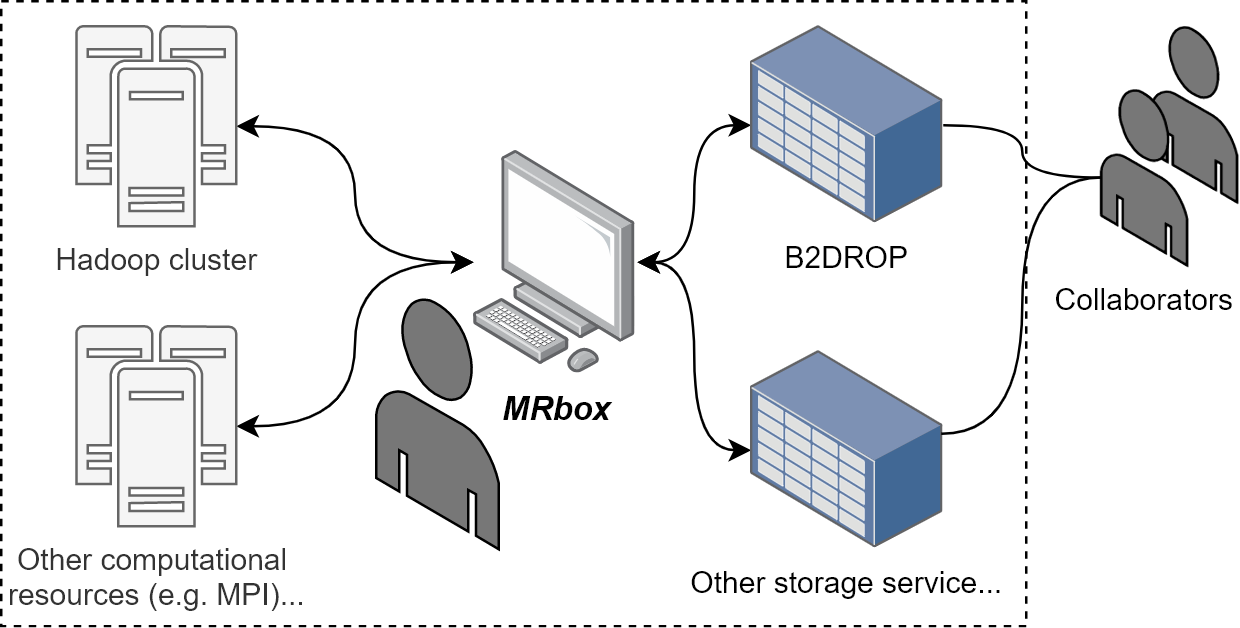
\includegraphics[width=.4\textwidth]{mrbox.png}
    \caption{The concept of MRbox is to simplify interacting with multiple analytics and big-data resources by extending the Cloud-storage paradigm.}
    \label{fig:mrbox}
\end{figure}

\section{Assumptions and Use-Cases}

For the development of MRbox, the two main assumptions made are: (i) Users do not necessarily have full control of the needed remote resources. They just have rights to create, delete, modify and relocate files in their remote folders and run computation jobs on them. (ii) When working with large and complex data sets, moving them should be avoided unless necessary\cite{atkinson_malcolm_2018}.

For the development of the current prototype, the following use cases were identified. Firstly, users should easily connect to the integrated remote infrastructures, just by running the MRbox application. Secondly, they need to have a complete view of the file system hierarchy in the remote resources from their local file system. When a remote data set exceeds in size the maximum file size that can be replicated in the local machine, a \texttt{link} file will be created locally, containing only the path to the remote file. Thirdly, users of MRbox would have a live preview of the files residing in a remote source by running file system commands in their terminal (e.g. \texttt{head}, \texttt{tail}), even when the files do not exist physically in the local machine. Moreover, users should be able to schedule computation jobs that will be executed in remote processing infrastructures by referring to files as if they were local. Lastly, users need to have seamless access to the output files generated by the scheduled jobs in order to do further analysis, or share them with their peers.

\section{System Overview}
This section summarises the main components and features of the application.

\subsection{A Sample Session With and Without MRbox}
As an example, let us consider the scheduling of a Map-Reduce job, which is the currently supported computation job. In the table below we compare the set of actions that a user needs to perform, with and without using MRbox.

\vspace{.5em}\noindent
\begin{tabular}{p{0.45\linewidth}|p{0.45\linewidth}}
    %\hline 
    \textbf{Using MRbox} & \textbf{Without Using MRbox} \\
    \hline
        1. Code the Map and Reduce functions locally. & 1. Code the Map and Reduce functions locally.\\ 
        2. Move the input file (or a $\texttt{link}$ to it) in the local $\texttt{MRbox}$ folder, if it is not already there. & 2. If the input data set is in the local file system, copy it to an HDFS cluster via HDFS terminal commands. If it is on a remote resource, use the resource-specific API or instructions to copy it to HDFS. \\ 
        3. Create a $\texttt{yaml}$ file specifying the local paths to Map and Reduce functions, input file and desired output location. Move the $\texttt{yaml}$ file in the local $\texttt{MRbox}$ folder. & 3. Use the Hadoop Streaming API to run the job. Move and generally manage the files generated using the HDFS commands as needed. \\
    \hline
        Outputs are automatically synced in the local $\texttt{MRbox}$ folder and in B2DROP. Links are created if the files are larger than a predefined size. & Use HDFS terminal commands to fetch the outputs locally. Use an ownCloud client or API to copy them to B2DROP. \\
    %\hline
\end{tabular}

\subsection{Supported Resources}
MRbox currently assumes a UNIX clone as the local and host system and supports the Apache Hadoop framework \cite{hadoop} and the B2DROP service \cite{b2drop}.

Apache Hadoop is a widely-used and open-source Map-Reduce framework. It includes two main modules; Hadoop Distributed File System (HDFS) and the Hadoop MapReduce. HDFS is the distributed file system primarily used by Hadoop applications, providing high data access performance, fault tolerance and native support of large data sets. MRbox establishes a connection to the desired HDFS on a remote cluster and it interacts with Hadoop MapReduce via the Hadoop command line tools provided.

B2DROP\cite{b2drop} is a user-friendly data synchronisation and exchange service created by the European Data Infrastructure (EUDAT\footnote{\url{https://eudat.eu/}}) for research communities. It provides a secure storage environment for long-tail but still volatile data that are subject to active research, while facilitating the process of sharing and keeping them up-to-date across different machines. It offers up to 20GB of storage per user. B2DROP offers automatic synchronisation via ownCloud\footnote{\url{https://owncloud.com/}}, an open source file synchronisation and sharing tool. Alternatively, the service can be accessed on the Web via an intuitive user interface, or on the local machine via a WebDAV Client.

\subsection{MRbox Configuration}
To connect to a remote HDFS, the local host needs to be configured as a client node. This usually requires to have a copy of the Hadoop distribution locally available and configured to access the remote cluster\cite{hadoopinst}. In \texttt{MRbox.conf} -- the configuration file of MRbox -- the user needs to specify the host and port of the HDFS NameNode, as well as the path to the local Hadoop installation. The user can also determine the absolute path of the local and HDFS folders that will be in sync, and the maximum size of the files that will be retrieved locally once created in an integrated remote resource. Depending on the distribution policy for MRbox, the Hadoop part of the configuration may also be pre-configured, therefore saving the end-user from even being aware of the connection specifics to the remote Hadoop cluster.

In addition, the B2DROP service is currently used by installing on the local machine the ownCloud Desktop Synchronisation Client following the B2DROP documentation. Both B2DROP and MRbox monitor the same local folder. A more fine-grained integration of ownCloud in MRbox will be developed in the future, e.g. by modifying the existing client.

\subsection{Managing Files}
MRbox creates folders locally and on the integrated remote resources, under the root paths specified in the \texttt{MRbox.conf} file. In order to keep track of local and remote instances of files and to promote consistency, MRbox implements a catalogue. This section describes this catalogue, how it stores mappings of local paths to remote ones, the synchronisation process between the local \texttt{MRbox} folder, HDFS and B2DROP, the implementation of links to comply with local size constraints, and the use of checksums for data validation.

\subsubsection{The Local Catalogue}

The local catalogue is used to maintain mappings between local and remote files and directories. In the current prototype of MRbox, the local catalogue maps the local paths to the paths of the corresponding files and directories on HDFS, making it possible for the user to interact with the HDFS of a remote cluster through the local file system hierarchy. Its current implementation is in SQLite\cite{sqlite}, a lightweight, self-contained SQL database engine that does not require a separate server process to operate and therefore is integrated in the application itself. For each file and folder, a record is created in the database consisting of the path, the most recent modification time and the checksum of the local and respective copy on HDFS. Each record also has an attribute specifying whether the local object is a file, a link (see Section \ref{sec:links}) or a directory.

\subsubsection{Synchronisation}
Synchronisation between the local \texttt{MRbox} folder and HDFS is one-way as we can only monitor the local folder for changes. Our current implementation makes use of the Python Watchdog library \cite{watchdog}, which monitors a designated local folder for changes. Depending on the type of the event identified, one of the following actions will take place: 
\begin{itemize}
    \item \texttt{on\_created()}: When a file, link or directory is created locally, it is registered in the local catalogue. For the case of file or directory, a copy is created on the remote HDFS. If the file created has a \texttt{.yaml} extension, MRbox attempts to run a Map-Reduce job on the remote Hadoop cluster, according to the specification passed in the \texttt{yaml} file (Figure 2). 
    \item \texttt{on\_deleted()}: When a file, link or directory is deleted locally, MRbox deletes the corresponding HDFS file and the record from the local catalogue.
    \item \texttt{on\_modified()}: When a file is modified locally, the HDFS file is modified accordingly and the local and HDFS checksums on the local catalogue are updated.
    \item \texttt{on\_moved()}: When a file, link or directory is moved within the local \texttt{MRbox} folder, the corresponding file or directory is relocated accordingly within the HDFS folder. 
\end{itemize}

\paragraph{Handling Bidirectional Synchronisation}
As discussed above, the current prototype assumes that users do not necessarily have full control over the remote resources. This means that, if files on HDFS change by any means other than through interacting with MRbox, MRbox will not have a way to track these changes, therefore leading to inconsistencies. To handle such potential inconsistencies between the local and HDFS \texttt{MRbox} folders an offline synchronisation process should be scheduled to run periodically. This is left for future work as low priority, since MRbox's main goal is to provide local views on remote HDFS resources, hiding direct access from its users.

In the case of B2DROP, bidirectional synchronisation is achieved through its desktop client, which is installed locally (Figure 2). To support special functionalities of MRbox (e.g. links, see below), this client would have to be modified further.

\subsubsection{Links}
\label{sec:links}
In MRbox, links are a special read-only file type recognised by the \texttt{.link} extension and registered in the local catalogue. Links are created to comply with local file size restrictions when large data sets are generated on the HDFS cluster and need to be made available locally. In the current prototype such files are the outputs of Map-Reduce jobs on HDFS.

The local file size limit can be specified in the MRbox configuration. After the completion of a Map Reduce job, the local file size limit is compared against  the size of the output file produced on HDFS. If the generated file is larger than the maximum allowable size limit, a \texttt{link} file is created, which contains the path to the remote file. This link can also be used in the browser to view the file on HDFS, if this is supported by the remote cluster. Moreover, if a \texttt{link} is deleted or moved within the local \texttt{MRbox} folder, the corresponding remote file will be deleted or moved respectively.

\paragraph{Synchronisation of Links Between B2DROP and HDFS}
In the current prototype, a link file in the local MRbox folder is synchronised verbatim onto B2DROP. However, this is not always desirable, since users would expect the complete file to be available on a data-exchange resource such as B2DROP. After all, the users that need to access a file on B2DROP may not have access to the HDFS cluster where it was created. To allow for special synchronisation treatment for the case of large files that appear as links locally, a customised synchronisation client would need to be implemented.

\subsubsection{File Checksums}
Checksums are used to guarantee data integrity in file transfers between the local and HDFS folder. HDFS uses a 32-bit cyclic redundancy check based on the Castagnoli polynomial (CRC32C). To perform end-to-end client side validation, MRbox adopts the composite CRC file checksum introduced in Apache Hadoop 3.1.1 that can be configured by setting \texttt{dfs.checksum.combine.mode} to \texttt{COMPOSITE\_CRC}. The composite CRC checksum is not applicable to links and directories. In contrast to Hadoop's default MD5 of MD5 of CRC file checksum computed across chunks and blocks, the composite CRC is independent of chunk and block configurations and describes only the logical file contents. As a result, it permits comparison between striped and replicated files, between HDFS instances with potentially different chunk and block size configurations, as well as between HDFS and local files or other external storage systems that implement Hadoop's File System interface \cite{googlecloudcrc,hadoopcrc}. At the end of each transfer, local file checksums are computed and compared against the checksums computed on HDFS. If the checksums do not match, the transfer will be repeated.

\subsection{Scheduling Map-Reduce Jobs}
MRbox aims to highlight the simplicity of the Map-Reduce model by hiding the technical implementation details from users. To trigger a Map-Reduce job users need to:
\begin{itemize}
    \item 
    Implement the Map and Reduce functions in two distinct files locally. Any programming language supported by the Hadoop Streaming utility can be used \cite{hadoopstreaming}.
    \item 
    Specify in a \texttt{yaml} file the absolute paths of the mapper and reducer scripts in the local file system. Also, users need to define the relative paths of the input as well as the output location. The input path can point to a file or a link. All paths are local and users do not need to know the file structure of the remote HDFS cluster.
    \item Move or save the \texttt{yaml} file in the local \texttt{MRbox} folder to trigger the execution.
\end{itemize}

MRbox will automatically issue the configured Map-Reduce job to the remote Hadoop using the Hadoop Streaming utility. The outputs will be fetched locally in the specified output path as files or links. The ownCloud Desktop Client, will replicate the output file to B2DROP, giving the user the possibility to share it with people working on the same project.

\subsection{Additional Tools}
The current prototype enables users to get a live preview of data sets residing on HDFS, by running \texttt{mrview.py cmd path} for a file, link or directory in the local \texttt{MRbox} folder. If the specified path corresponds to a file or directory, the supported UNIX command is executed. If the path corresponds to a link, the data set does not exist locally due to size constraints. Users can run \texttt{head} and \texttt{tail} commands to get an overview of the HDFS data corresponding to the link. The list of supported commands for links can be extended to a complete suite of tools in the future.

\begin{figure}
  \centering
  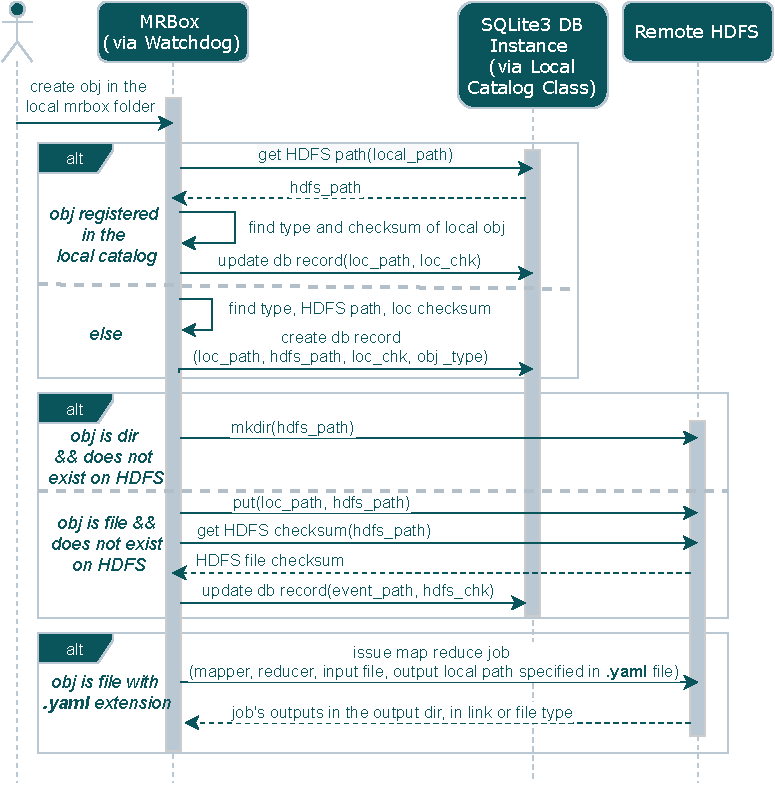
\includegraphics[width=\linewidth, height=8cm]{on_created_seq_sys.pdf}
  \caption{Sequence of events after a file is created in the local $\texttt{MRbox}$ folder}
\end{figure}

\section{Related Work}
Scientific and business workflow management systems and Workflow-as-a-Service platforms \cite[etc.]{kepler,pegasus,dare} often facilitate the processing of big data across multiple e-infrastructures. However, only a limited number of them integrate big data frameworks, such as Hadoop, directly, without focusing on a certain data organisation or field-specific problems \cite{wang2009kepler}. In addition, these systems still present challenges for big data analytics in the cloud and when used across organisations with potentially heterogeneous resources and execution environments \cite{khan2019big}. As a result, the data-operations that need to be performed are partially automated and professionals have to manually configure and use the involved services and local and remote infrastructures. Finally, identifying whether a workflow supports a specific data lake, platform or tool is usually a challenging task and users need to get familiar with a new Graphical User Interface (GUI) and the specific workflow model to efficiently use the management system \cite{khan2019big, wang2009kepler}. In contrast to workflow management systems, MRbox does not require that its users learn a new GUI or a workflow model specification language.

Furthermore, MRbox borrows from and extends cloud storage, synchronisation and data exchange services, such as Dropbox. However, apart from synchronising files and folders and allowing users to share their data, MRbox investigates the extension of this interaction paradigm for data analytics and distributed processing, as well as for synchronising amongst multiple resources.

\section{Conclusions and Future Work}
For the processing and sharing of big data, researchers and data analysts use a plethora of tools and heterogeneous infrastructures. As a result, performing data-intensive tasks is typically non-automated and arduous and requires technical knowledge of the underlying systems. MRbox aims to lower the barrier of technical expertise by hiding the complexity of big data technologies from non-experts. Using the file system hierarchy of the local operating system, MRbox provides a unifying view of local and remote resources and the data residing in them, and enables users to schedule computational jobs on remote infrastructures as if they were local. In the current prototype, Hadoop and B2DROP services are supported and Map-Reduce jobs can be scheduled.

This work can be improved in several ways. Firstly, we need to test MRbox under heavier workloads. A more fine-grained integration of ownCloud in MRbox will be implemented to enable users to directly connect to the B2DROP service without installing a separate client. Secondly, the ownCloud client needs to be modified and expanded further to support special functionalities of MRbox, e.g. for the case of links, the complete data set should be available on resources such as B2DROP. Thirdly, according to a distribution policy, the connection to remote infrastructures, such as a Hadoop cluster, could be pre-configured, saving the end-user from even being aware of the configuration specifics. Additionally, to verify our concept, we have to measure the usability and performance of the current prototype among potential users that want to perform different types of workloads. Furthermore, while maintaining simplicity, we will investigate expanding to other resources and execution contexts, e.g. triggering the execution of numerical codes on MPI clusters. 

A valuable more theoretical follow-up work could be the formalisation of resource types and integration policies, which will add to the extensibility of MRbox while minimising the risk of data inconsistencies and resource mismanagement. This approach could lead to future research towards a more general framework, which incorporates heterogeneous computational services and storage resources for big data analytics via localised views. An alternative direction could be the exploitation of the unifying files-based view of heterogeneous resources to integrate widely used tools and UIs, e,g, spreadsheet applications to transparently make use of large data sets on remote HDFS clusters.

%\begin{acks}
%\end{acks}

\bibliographystyle{ACM-Reference-Format}
\bibliography{mrbox}

\end{document}
\endinput